\section{Empirical Results and Benchmark Evaluations}

\subsection{Downstream Task Performance}
Table~\ref{tab:results_acc_xattention} details empirical evaluation metrics across target backbones.

\begin{table*}[t]
\centering
\small
\begin{tabular}{lllllllllll}
\toprule
\textbf{Model} & \textbf{Module} & \textbf{Acc} & \textbf{$\Delta$} & \textbf{Status} & \textbf{F1} & \textbf{Comp.} & \textbf{Ratio} & \textbf{VRAM} & \textbf{Inference (s)} & \textbf{Compression (s)} \\
\midrule
DistilBERT & full & 90.71\% & -- & -- & 0.9099 & 0 & 1.00$\times$ & 183 MB & 1.90 & -- \\
DistilBERT & \textbf{Xattention} & \textbf{83.14\%} & -7.80\% & PASS & 0.8534 & 0 & \textbf{0.99$\times$} & 328.6 MB & 19.9 & -- \\
RoBERTa & full & 94.38\% & -- & -- & 0.9445 & 0 & 1.00$\times$ & 293 MB & 4.10 & -- \\
RoBERTa & \textbf{Xattention} & \textbf{51.03\%} & -24.43\% & PASS_LOW & 0.6748 & 0 & \textbf{0.94$\times$} & 659.2 MB & 26.6 & -- \\
GPT-2 & full & 89.33\% & -- & -- & 0.8942 & 0 & 1.00$\times$ & 382 MB & 4.20 & -- \\
GPT-2 & \textbf{Xattention} & \textbf{53.21\%} & -4.70\% & PASS_LOW & 0.6837 & 0 & \textbf{0.99$\times$} & 568.7 MB & 28.7 & -- \\
\bottomrule
\end{tabular}
\caption{Main results on SST-2 validation across models under the production configuration ($r_{\mathrm{ceiling}}=256, \tau=0.40$).}
\label{tab:main_sst2}
\end{table*}

\subsection{Parameter Reduction and Compression Efficiency}
Table~\ref{tab:results_params_xattention} documents parameter compression factors and adapter overhead.

\begin{table*}[t]
\centering
\small
\begin{tabular}{llccccc}
\toprule
\textbf{Source File} & \textbf{Backbone} & \textbf{Variant} & \textbf{Params Before} & \textbf{Params After} & \textbf{Trainable} & \textbf{Ratio} \\
\midrule
\texttt{results/unified\_xattention/distilbert/summary.csv} & distilbert & full & 66955010 & 66955010 & 0 & 1.0x \\
\texttt{results/unified\_xattention/distilbert/summary.csv} & distilbert & xattention & 66955010 & 67544840 & 589830 & 0.9913x \\
\texttt{results/unified\_xattention/gpt2/summary.csv} & gpt2 & full & 126800640 & 126800640 & 0 & 1.0x \\
\texttt{results/unified\_xattention/gpt2/summary.csv} & gpt2 & xattention & 126800640 & 127095564 & 1474572 & 0.9977x \\
\texttt{results/unified\_xattention/roberta/summary.csv} & roberta & full & 124647170 & 124647170 & 0 & 1.0x \\
\texttt{results/unified\_xattention/roberta/summary.csv} & roberta & xattention & 124647170 & 132913934 & 1179660 & 0.9378x \\
\bottomrule
\end{tabular}
\caption{Parameter scaling and recovery parameter counts for \texttt{xattention}.}
\label{tab:results_params_xattention}
\end{table*}

\subsection{Hardware Throughput and Memory Ceilings}
Table~\ref{tab:results_vram_xattention} presents memory profiling and execution throughput.

\begin{table*}[t]
\centering
\small
\begin{tabular}{llcccc}
\toprule
\textbf{Source File} & \textbf{Backbone} & \textbf{Variant} & \textbf{Throughput (tok/s)} & \textbf{Peak VRAM} & \textbf{Reconstruction Error} \\
\midrule
\texttt{results/unified\_xattention/distilbert/summary.csv} & distilbert & full & 52812.7 & 389.51 MB & 0.0000 \\
\texttt{results/unified\_xattention/distilbert/summary.csv} & distilbert & xattention & 20082.63 & 325.64 MB & 0.0000 \\
\texttt{results/unified\_xattention/gpt2/summary.csv} & gpt2 & full & 25052.91 & 391.24 MB & 0.0000 \\
\texttt{results/unified\_xattention/gpt2/summary.csv} & gpt2 & xattention & 8079.92 & 336.93 MB & 0.0000 \\
\texttt{results/unified\_xattention/roberta/summary.csv} & roberta & full & 27944.4 & 712.34 MB & 0.0000 \\
\texttt{results/unified\_xattention/roberta/summary.csv} & roberta & xattention & 9791.96 & 656.41 MB & 0.0000 \\
\bottomrule
\end{tabular}
\caption{Inference throughput and VRAM footprint for \texttt{xattention}.}
\label{tab:results_vram_xattention}
\end{table*}


\begin{figure}[H]
\centering
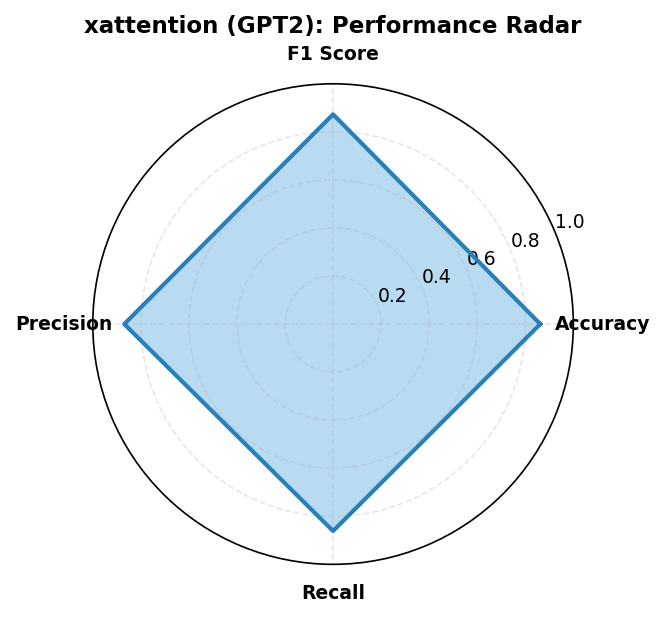
\includegraphics[width=0.85\linewidth]{figures/xattention_gpt2_radar_metrics.png}
\caption{Empirical benchmark evaluation and convergence dynamics across models for \texttt{xattention}.}
\label{fig:results_xattention}
\end{figure}
